\documentclass[11pt,a4paper]{article}
\usepackage{fontspec}
\setmainfont{TeX Gyre Pagella}
\newfontfamily\headfont{Inter}[UprightFont=*-ExtraBold,BoldFont=*-ExtraBold,Extension=.otf,Path=/usr/share/fonts/opentype/inter/]
\usepackage[a4paper,margin=2.3cm]{geometry}
\usepackage{graphicx}
\graphicspath{ {../blog/} }
\usepackage{booktabs,float,caption,array,xcolor}
\usepackage[hidelinks]{hyperref}
\usepackage{titlesec}
\usepackage{setspace}
\usepackage[round]{natbib}
\setstretch{1.05}
\renewcommand{\topfraction}{0.9}
\renewcommand{\bottomfraction}{0.8}
\renewcommand{\textfraction}{0.1}
\renewcommand{\floatpagefraction}{0.75}
\setlength{\parindent}{0pt}
\setlength{\parskip}{0.55em}
\titleformat{\section}{\headfont\Large}{\thesection}{0.8em}{}
\titleformat{\subsection}{\headfont\large}{\thesubsection}{0.8em}{}
\captionsetup{font=small,labelfont=bf}
\urlstyle{same}
\hypersetup{pdftitle={The Earth at Night},pdfauthor={Tristan Hotham}}

\begin{document}
\begin{center}
{\Large\bfseries The Earth at Night\\[2pt] Where the World Lit Up and Where It Went Dark, from Satellite Night Lights 2012 to 2024\par}
\vspace{1.2em}
{\large Tristan Hotham\par}
\vspace{0.3em}
{\small Independent researcher\\
ORCID: 0000-0003-4931-9349\\
DOI: 10.5281/zenodo.23857868\par}
\vspace{0.8em}
2026
\end{center}

\begin{quote}
\small
\begin{center}\textbf{Abstract}\end{center}
I measure how the world's artificial light at night changed between 2012 and 2024, using the Annual VIIRS Night Lights (VNL) V2 as prepared by Hengl in a consistent yearly stack, summed as radiance times area over countries, World Bank regions and the 20 km around 1,007 cities of at least half a million people. After correcting a tenfold change of storage scale between the 2021 and 2022 layers of that release, the light seen from space rose by 57\% between 2012 and 2024 (41\% between the three-year averages at either end), and the land area that averaged at least 1 nW/cm²/sr grew by 61\%. China and India gave 26\% of the increase; South Asia's light grew fastest of any region (159\%), while sub-Saharan Africa, home to 14\% of the world's people, still gave off only 2.6\% of its light. Of 141 countries with at least a million people, 47 at least doubled their light, led by Nepal (9.3 times), Cambodia (7.0) and Ghana (6.4), and 17 lost light. The deepest falls follow war (Ukraine 73\% between 2021 and 2022; Syria, Yemen, and Khartoum after 2023) and economic or power crises (Lebanon 71\% between 2019 and 2022; Venezuela 41\% between 2014 and 2020). A third group of falls, in France (-40\%), the Netherlands and the United Kingdom, most likely reflects the change from sodium lamps to LEDs, to which the sensor is partly blind, and lights switched off after midnight, not a darker night on the ground. Modelled years back to 2000 are shown for orientation only; they do not join the observations.

\textbf{Keywords:} night lights; VIIRS; Day/Night Band; artificial light at night; electrification; conflict; LED street lighting; light pollution; remote sensing; open data
\end{quote}

\section{Introduction}
Satellite images of the Earth at night have become one of the most familiar pictures of human settlement, and since the work of \citet{henderson} on measuring economic growth from outer space, one of the most used proxies in economics and development research. Since 2012 the Visible Infrared Imaging Radiometer Suite (VIIRS) Day/Night Band, on satellites that pass every place at about 1.30 am local time, has measured night light with calibrated radiances and far less saturation than the older DMSP sensors \citep{elvidge2017}. The Earth Observation Group's Annual VIIRS Night Lights (VNL) V2 turn the monthly composites into yearly averages from which fires, aurora and background noise are filtered \citep{elvidge2021}.

This study asks three simple questions of those annual averages. How much brighter is the planet in 2024 than in 2012? Where did the new light come from? And where did the light go out, and why? It uses the open, consistent yearly stack prepared by \citet{hengl}, which also extends the series back to 2000 with a statistical model, and the DMSP-style long-term average from the same source, after \citet{li2020}. An interactive map (\url{https://maps.tristanhotham.com/earth-at-night/}) shows every year, a swipe between any two years, the change from 2012 to 2024 and the long-term average.

\section{Data}
Table~\ref{tab:sources} lists the sources. \citet{hengl} publishes the VNL V2 annual averages for 2012 to 2024 at 500 m (15 arc seconds), converted from the original radiance in nW/cm²/sr to tenths of a nW and stored as Cloud-Optimised GeoTIFFs, together with layers for 2000 to 2011 extrapolated backwards by a per-pixel logistic regression, principal components of the series, a 2000 to 2024 difference layer and a DMSP-style 1 km stack for 1992 to 2024. I used overview levels built into those files: 2,700 by 1,120 cells for every year (2 arc minutes, about 14.8 km at the equator) and 5,400 by 2,240 for 2012 and 2024 (about 7.4 km). The extent, longitude 180° W to 180° E and latitude 87.37° N to 62.0° S, was checked by moving the grid by a tenth of a degree and confirming that Natural Earth's large cities fall on the brightest light at the stated position. The DMSP-style layer is an average over 1992 to 2024 at 30 arc seconds, extending from 75° N to 65° S (checked the same way against VIIRS, correlation 0.70 in logarithms). Countries, populations (POP\_EST, mostly for 2019), World Bank regions and populated places come from Natural Earth.

\begin{table}[tbp]\centering\small\caption{Sources and licences.}\label{tab:sources}\begin{tabular}{>{\raggedright\arraybackslash}p{3.6cm}>{\raggedright\arraybackslash}p{7.6cm}>{\raggedright\arraybackslash}p{2.6cm}}\toprule Source & Used & Licence\\\midrule
VNL V2 annual night lights (EOG, Colorado School of Mines), via \citet{hengl} & Annual averages 2012 to 2024 at about 15 km (all years) and 7 km (2012, 2024); modelled years 2000 to 2011 & CC BY 4.0\\
DMSP-style lights, after \citet{li2020}, via \citet{hengl} & Average over 1992 to 2024, 1 km & CC BY 4.0\\
Natural Earth & Countries, POP\_EST, World Bank regions; 1,007 populated places of at least 500,000 people & Public domain\\
\bottomrule\end{tabular}\end{table}

\section{Methods}
\subsection{A scale change in the release}
On cells brighter than 5 nW in 2021, the ratio of the 2022 layer to the 2021 layer has a median of 0.100 (11,264 cells): the 2022, 2023 and 2024 layers of this release are stored in whole nW, not tenths. All years were therefore converted to whole nW and rounded to the nearest whole nW, so that the earlier years carry the same precision as the later ones, and negative values were set to zero. Rounding removes cells whose 15 km average is below 0.5 nW in every year alike. The 2012 to 2024 layers have no data north of 75.1° N; that strip is left out of every year, including the modelled ones.

\subsection{Light units, countries and cities}
Light is summed as radiance times area: a cell of $A$ km² averaging $v$ nW/cm²/sr contributes $vA$ light units. Each cell was given to the Natural Earth country holding most of its land, from a rasterisation at four by four sub-cells (two by two on the 7 km grid); cells with no land belong to no country. 1.9\% of the 2024 light falls outside every country (boats, platforms and coastal glare) and is counted only in the world total. Natural Earth's de facto borders put Crimea in Russia. Cities are Natural Earth populated places with at least 500,000 people; their light is the sum within 20 km of the point on the 7 km grid for 2012 and 2024 and on the 15 km grid for the yearly series, so neighbouring cities can overlap. Country rankings use the 141 countries with at least a million people and 2,000 light units in 2012; city rankings use the 443 cities with at least a million people whose disc averaged at least 2 nW in 2012. Light per person divides 2024 light by POP\_EST and scales the world average to 100. The deepest fall is the largest drop from an earlier peak within 2012 to 2024.

\subsection{Robustness}
Annual composites vary with cloud, snow, moonlight filtering and viewing geometry. Every change from 2012 to 2024 was recomputed between the averages of 2012 to 2014 and 2022 to 2024. The modelled years were summed the same way but play no part in any claim.

\section{Results}
\subsection{A brighter, more widely lit planet}
The world gave off 33.2 million light units in 2012 and 52.3 million in 2024, a rise of 57\% (Figure~\ref{fig:series}); between the three-year averages the rise is 41\%. The total fell from one year to the next only in 2014, 2015 and 2020. The lit area grew faster than the light: land averaging at least 1 nW covered 9.3 million km² in 2012 and 15.1 million km² in 2024 (61\% more), 6.8\% and 10.9\% of the land. These rates are in line with the growth of lit area and radiance reported for 2012 to 2016 by \citet{kyba2017}. The modelled series rises from 21.6 million units in 2000 to 24.9 million in 2011 and sits 34\% below the first observed year: it is a backwards extrapolation, not a measurement.

\begin{figure}[tbp]\centering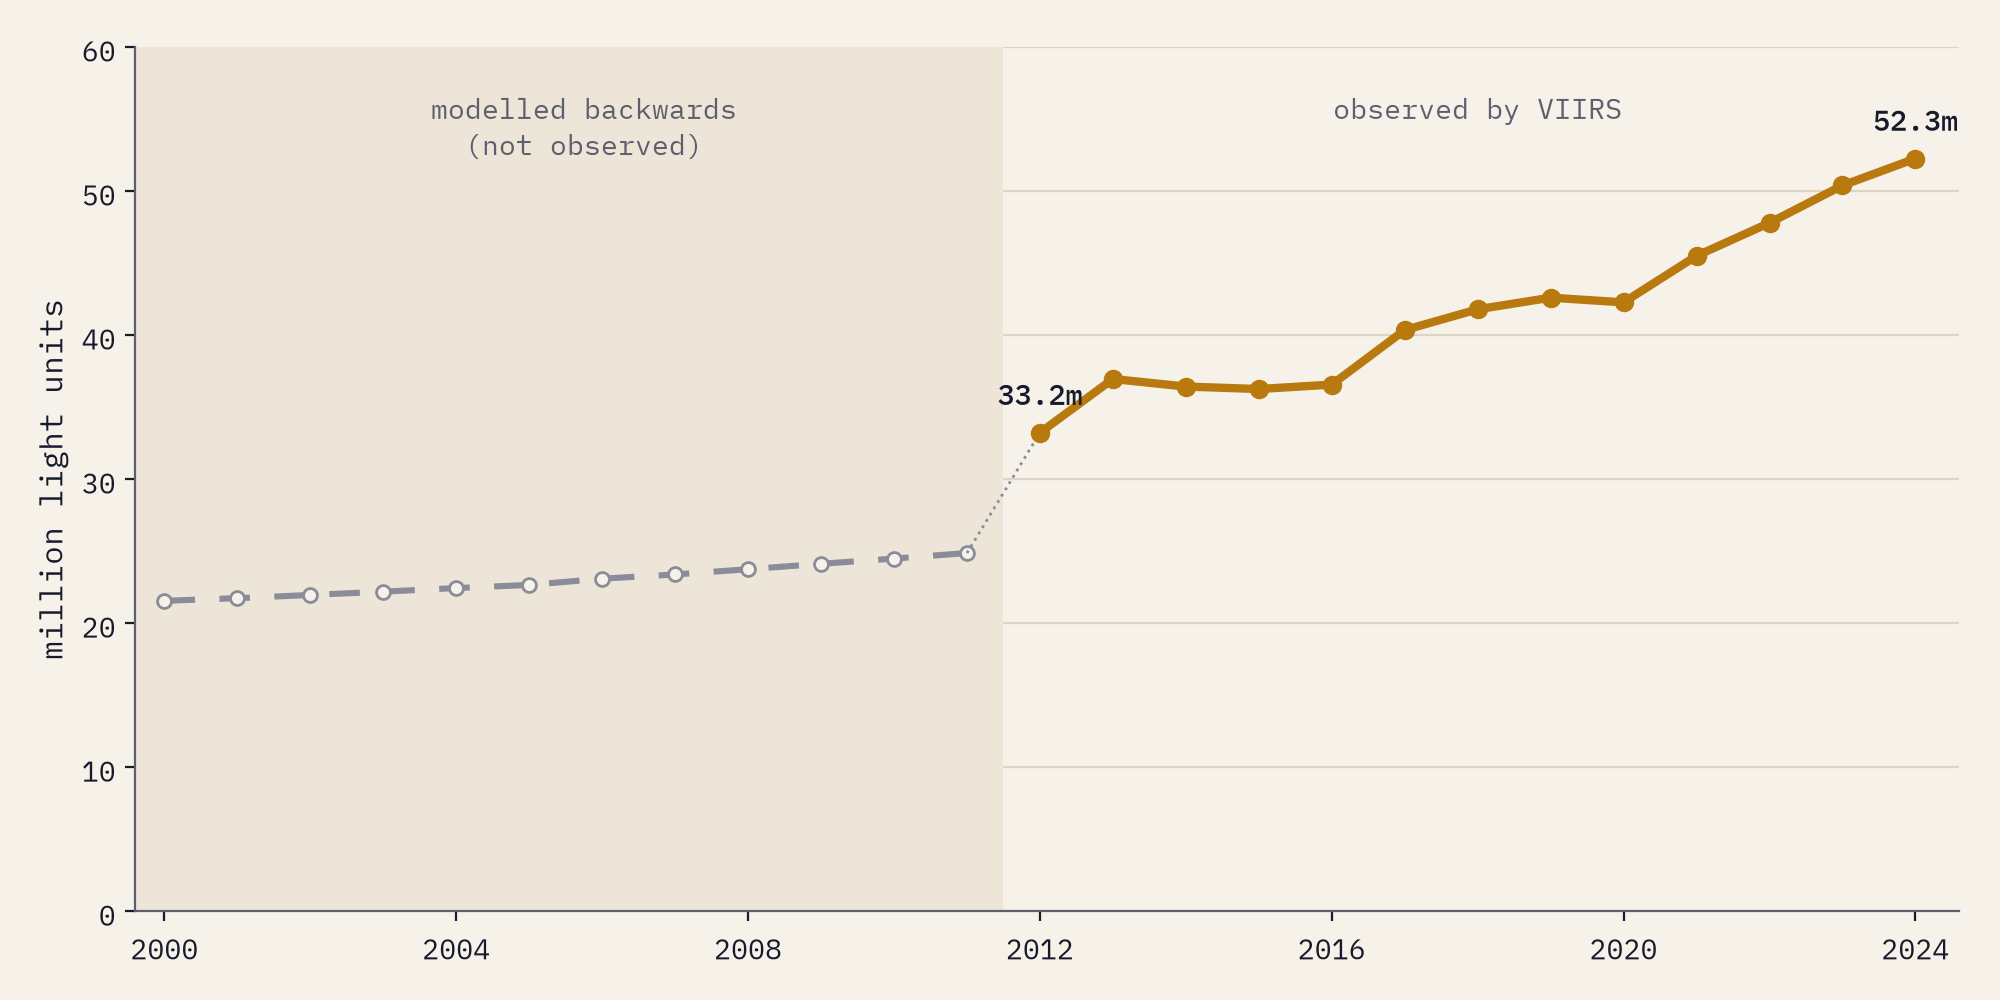
\includegraphics[width=.86\linewidth]{b_series.png}\caption{Total light each year on the 15 km grid. Solid: observed by VIIRS. Dashed, shaded: modelled backwards by \citet{hengl}.}\label{fig:series}\end{figure}
\begin{figure}[tbp]\centering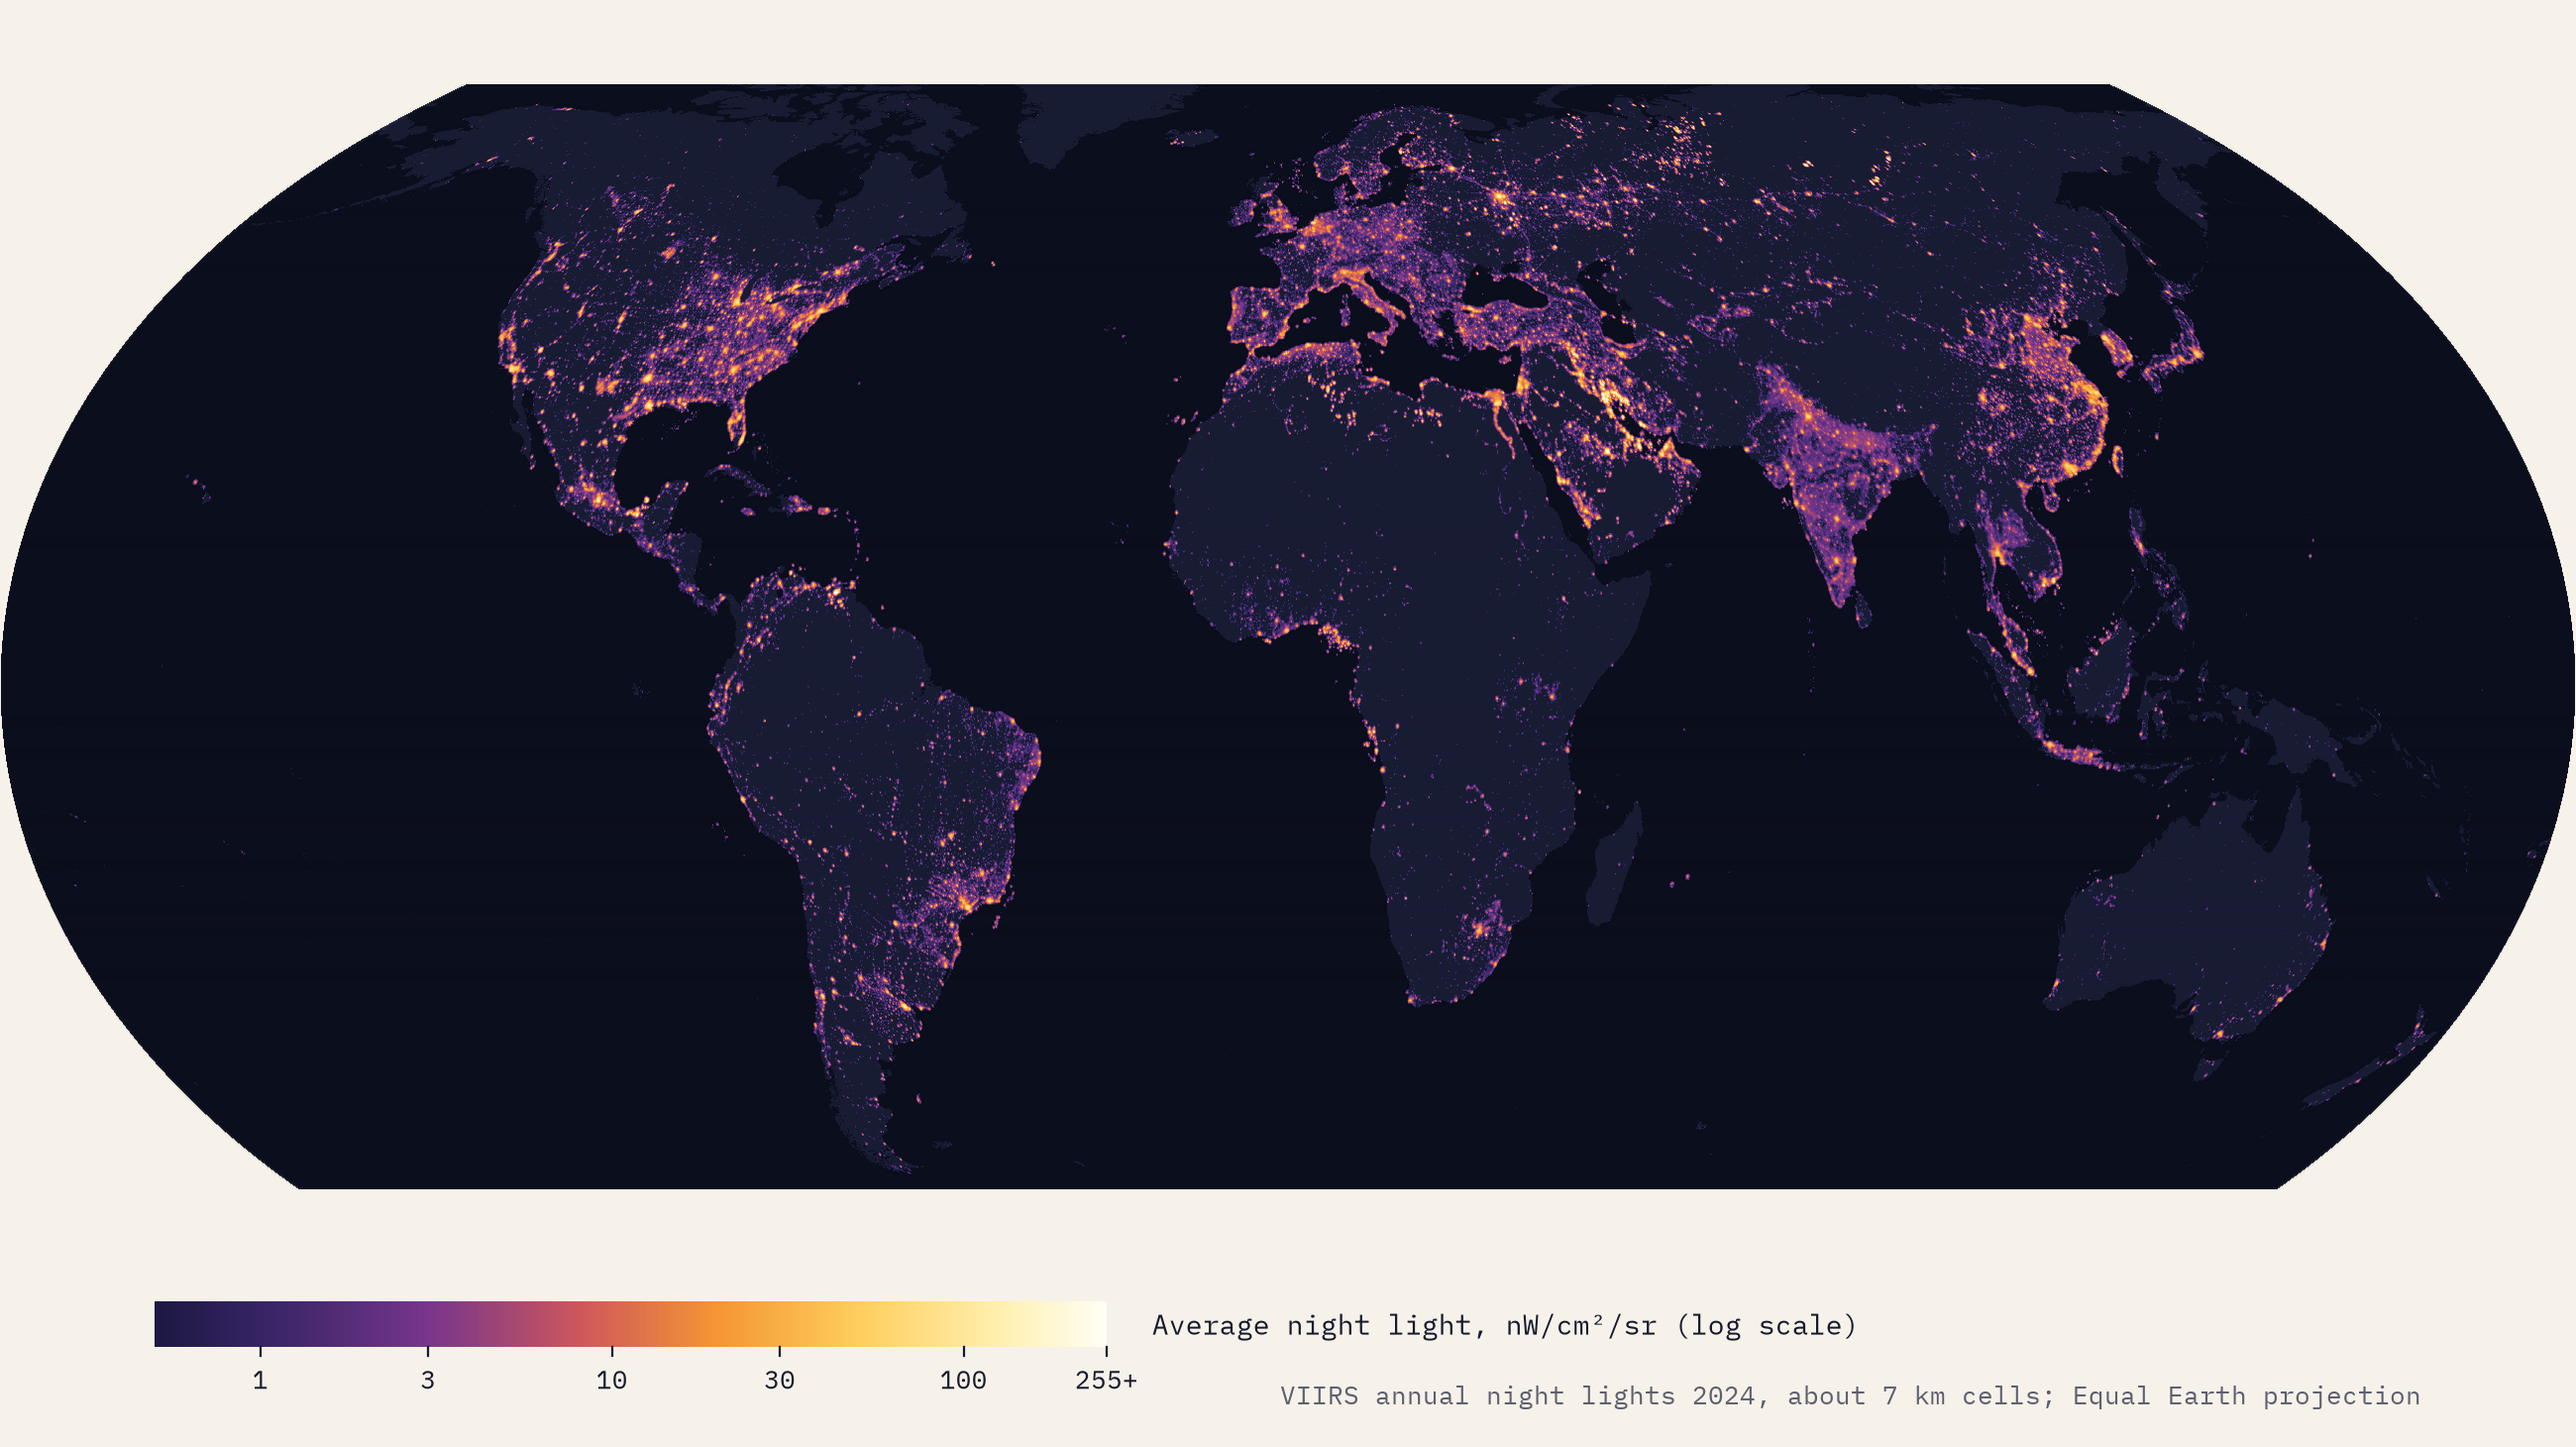
\includegraphics[width=\linewidth]{b_world_2024.png}\caption{Night lights in 2024 (VNL V2 via \citet{hengl}, 7 km grid, small lights given a soft halo so that they show at this scale), Equal Earth projection.}\label{fig:world}\end{figure}

The geography of light shifted east and south (Table~\ref{tab:regions}, Figure~\ref{fig:regions}). North America's share fell from 24.2\% to 18.7\% and Europe and Central Asia's from 26.6\% to 22.7\%, while East Asia and the Pacific rose from 14.7\% to 18.1\% and South Asia from 4.5\% to 7.4\%. Sub-Saharan Africa's light grew by 70\%, yet its share rose only from 2.4\% to 2.6\%, against 14\% of the world's people.

\begin{table}[tbp]\centering\small\caption{Light by World Bank region: millions of light units, change between single years and between three-year averages, share of world light and of people (\%), and light per person (world = 100).}\label{tab:regions}\setlength{\tabcolsep}{4pt}\begin{tabular}{lrrrrrrrr}\toprule Region & 2012 & 2024 & Change & 3-year & Share 2012 & Share 2024 & People & Per person\\\midrule
North America & 7.80 & 9.58 & +23\% & +11\% & 24.2 & 18.7 & 4.8 & 392\\
Europe and Central Asia & 8.60 & 11.65 & +36\% & +27\% & 26.6 & 22.7 & 12.0 & 189\\
East Asia and Pacific & 4.74 & 9.28 & +96\% & +75\% & 14.7 & 18.1 & 30.5 & 59\\
Middle East and North Africa & 5.07 & 9.25 & +82\% & +62\% & 15.7 & 18.1 & 6.0 & 303\\
Latin America and the Caribbean & 3.83 & 6.38 & +67\% & +41\% & 11.9 & 12.5 & 8.4 & 148\\
South Asia & 1.46 & 3.79 & +159\% & +120\% & 4.5 & 7.4 & 23.9 & 31\\
Sub-Saharan Africa & 0.78 & 1.33 & +70\% & +46\% & 2.4 & 2.6 & 14.5 & 18\\
\bottomrule\end{tabular}\end{table}
\begin{figure}[tbp]\centering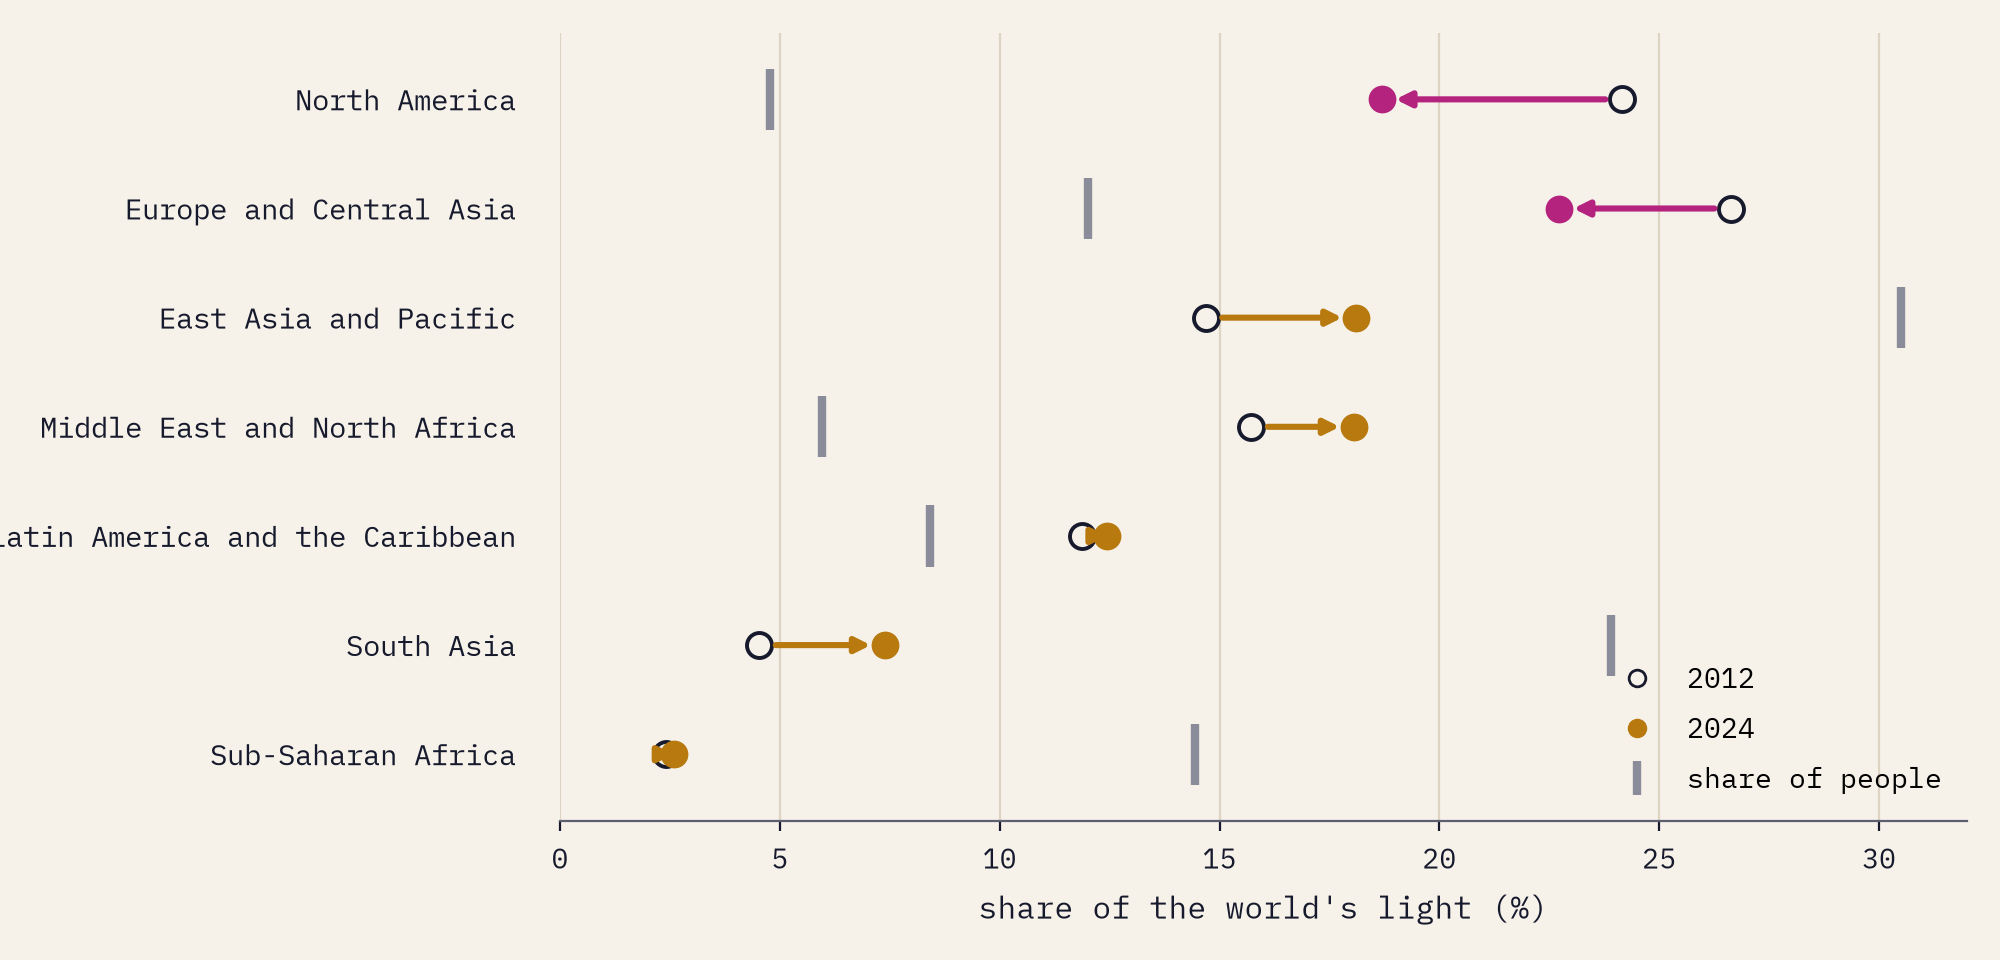
\includegraphics[width=.86\linewidth]{b_regions.png}\caption{Share of the world's light by World Bank region, 2012 and 2024, with each region's share of the world's people.}\label{fig:regions}\end{figure}

\subsection{Where the world lit up}
China's light grew 2.1 times and India's 2.7 times; together they account for 26\% of the global increase. China's share rose from 7.9\% to 10.5\% and India's from 3.9\% to 6.6\%; the United States remained the brightest country but its share fell from 21.6\% to 16.9\%. Of the 141 countries ranked, 47 at least doubled their light and 16 at least tripled it (Table~\ref{tab:up}, Figure~\ref{fig:countries}). The fastest growth was from low starting points: Nepal (9.3 times), where long daily power cuts ended between 2016 and 2018, Cambodia (7.0), Ghana (6.4), Tanzania (6.0), Côte d'Ivoire (5.5), Senegal (5.2), Kenya (4.9) and Ethiopia (4.2). Among cities of a million or more, Kumasi (4.4 times), Addis Ababa (3.6), Accra (3.3), Dar es Salaam (3.0) and Abidjan (3.0) stand out (Table~\ref{tab:cities}).

Some growth is not settlement. Iraq (3.2 times) and Iran (2.4) include oil fields where associated gas is flared, which VNL V2 keeps as light; the area around Basra grew 3.5 times. In Venezuela a box around the Monagas oil fields held 42\% of the country's light in 2012 and 53\% in 2024. No flare mask was available for this study, so country totals include flares.

\begin{table}[tbp]\centering\small\caption{The fifteen countries whose light grew fastest, 2012 to 2024 (thousand light units; countries with at least a million people and 2,000 units in 2012).}\label{tab:up}\begin{tabular}{lrrrrl}\toprule Country & 2012 & 2024 & Change & 3-year & Deepest fall\\\midrule
Nepal & 2.7 & 25.4 & +829\% & +762\% & 24\% (2015 to 2016)\\
Cambodia & 2.6 & 18.1 & +600\% & +441\% & 12\% (2013 to 2014)\\
Ghana & 21.4 & 136.1 & +535\% & +377\% & 3\% (2014 to 2015)\\
Kenya & 9.4 & 46.4 & +391\% & +270\% & 3\% (2019 to 2020)\\
Ethiopia & 5.2 & 22.1 & +325\% & +188\% & 12\% (2017 to 2018)\\
Armenia & 3.9 & 15.6 & +304\% & +192\% & 36\% (2013 to 2015)\\
Mauritania & 2.3 & 8.7 & +282\% & +215\% & 3\% (2019 to 2020)\\
Laos & 3.6 & 13.2 & +270\% & +189\% & 10\% (2018 to 2019)\\
Uganda & 4.2 & 14.7 & +253\% & +219\% & 16\% (2012 to 2013)\\
\bottomrule\end{tabular}\end{table}
\begin{figure}[tbp]\centering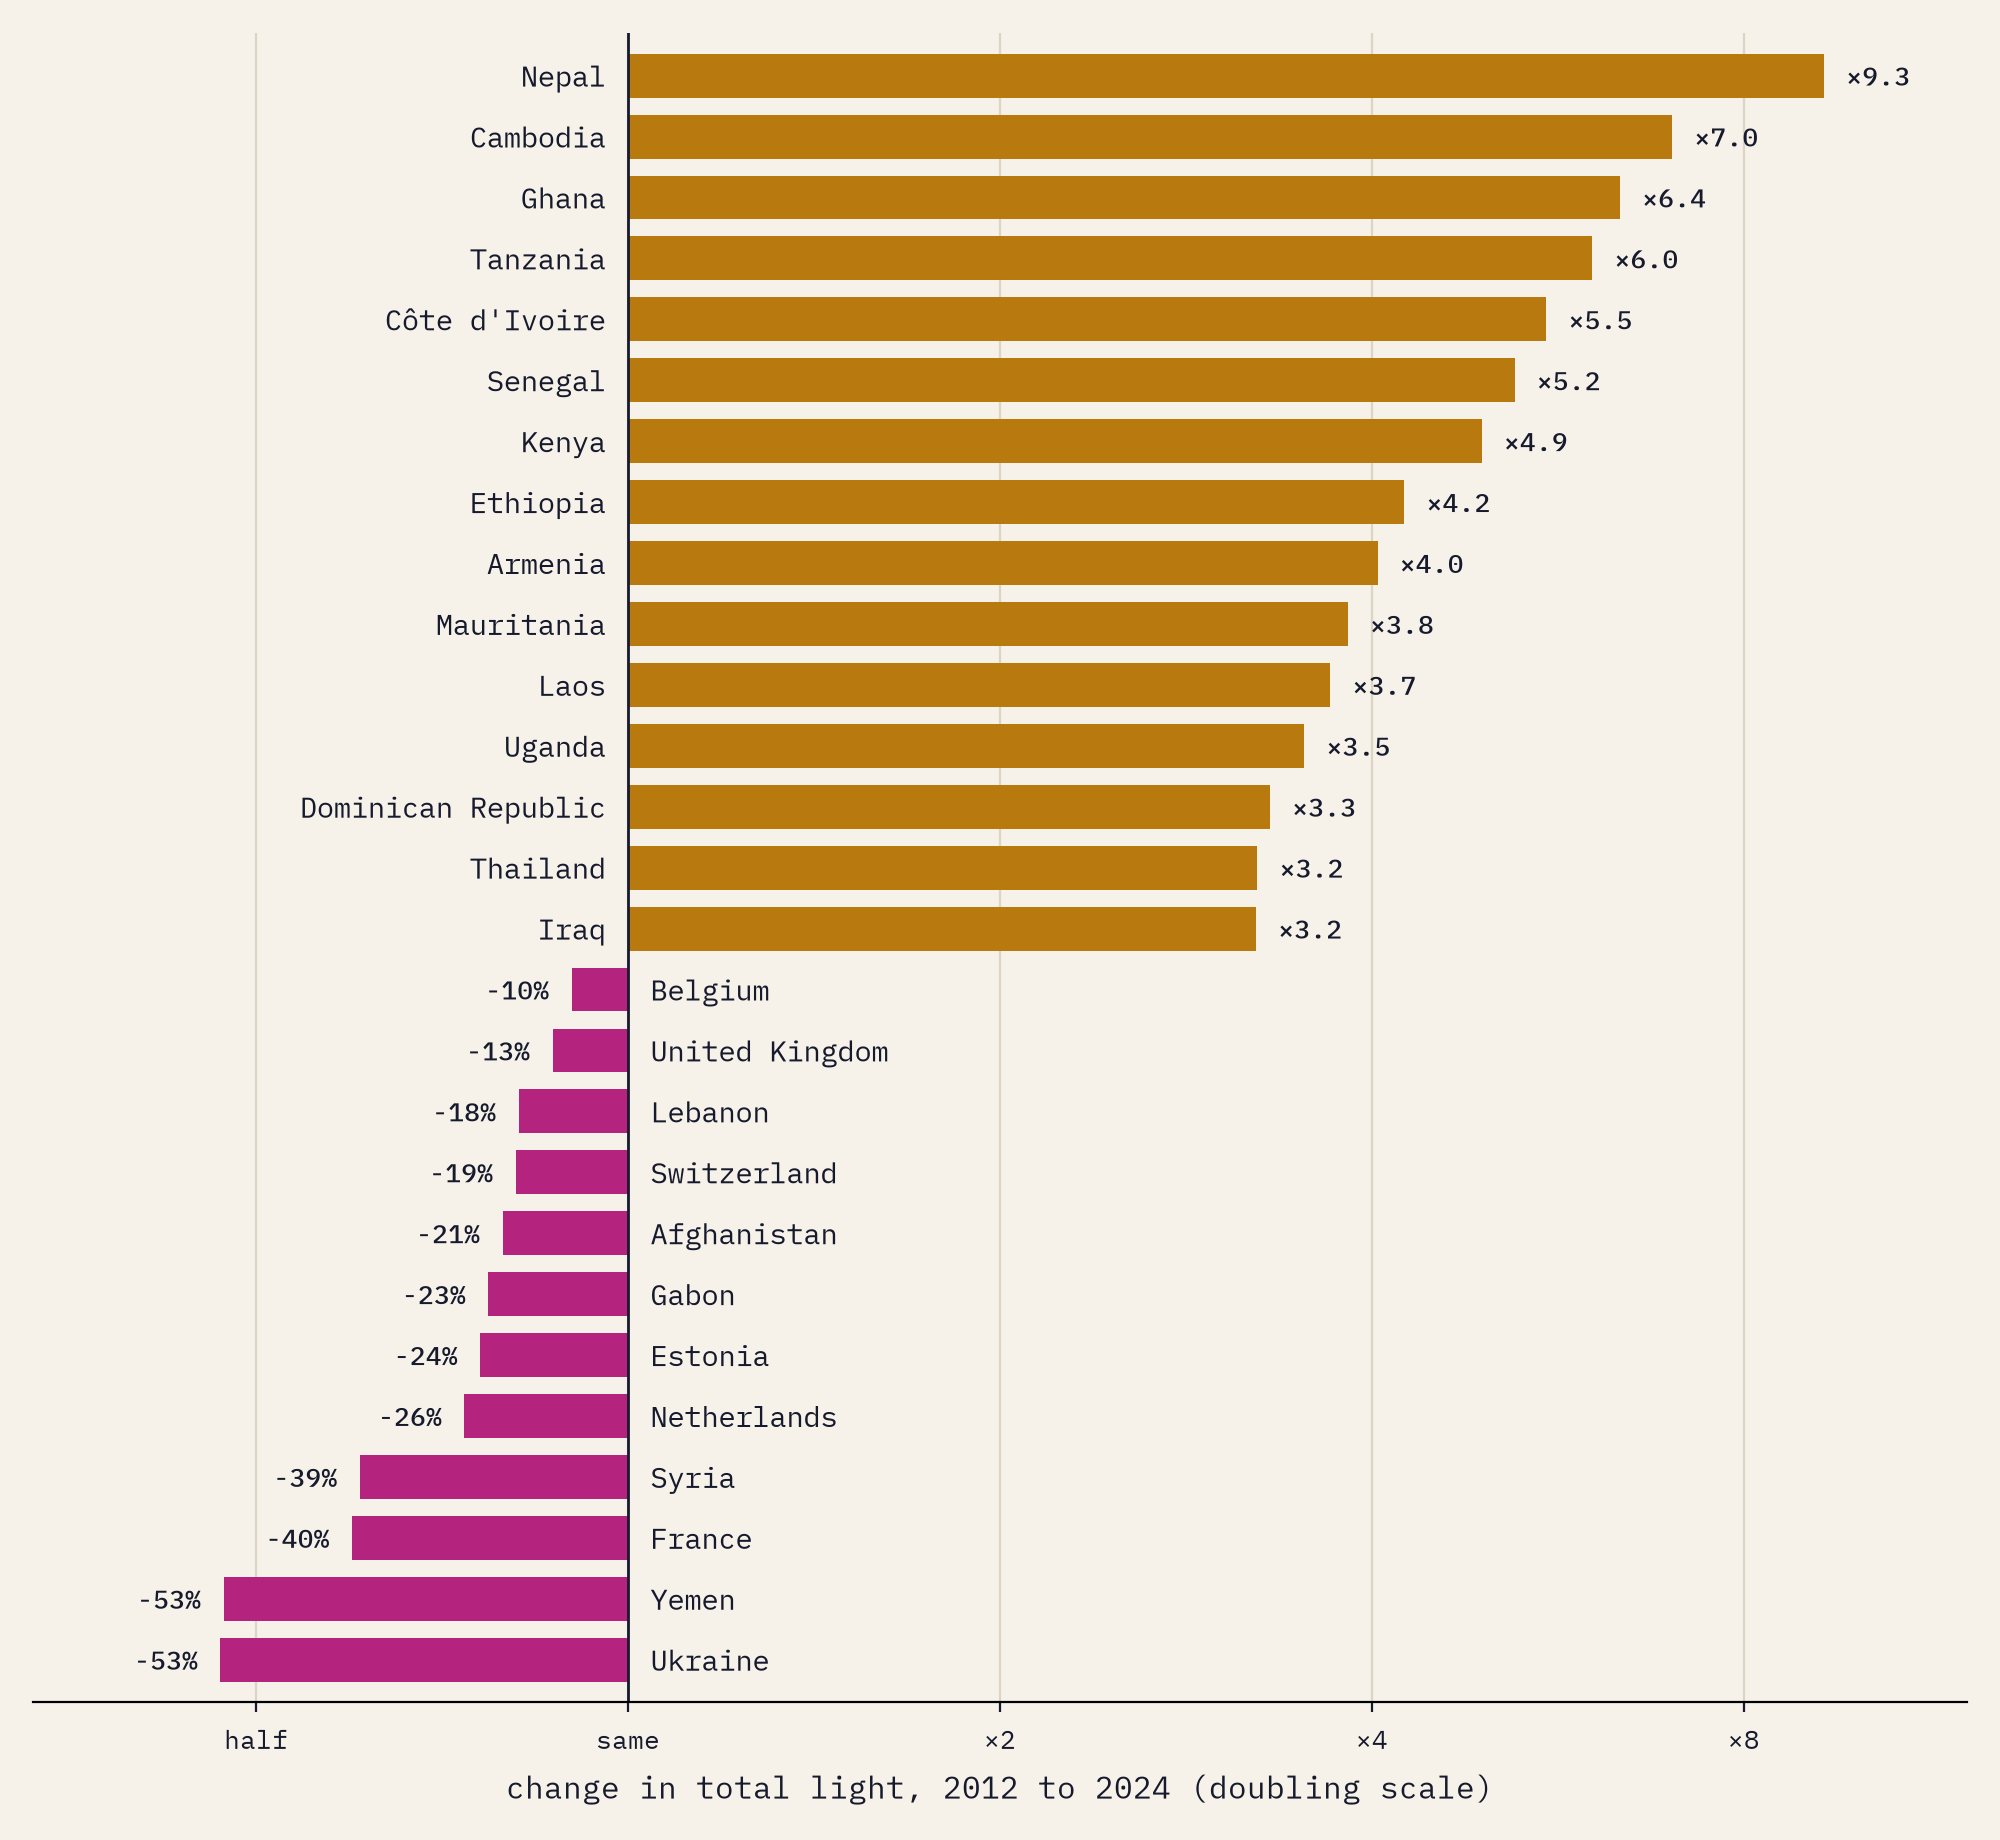
\includegraphics[width=.82\linewidth]{b_countries.png}\caption{Change in total light, 2012 to 2024, for the fifteen fastest risers and every country that lost a tenth or more of its light (countries with at least a million people and 2,000 light units in 2012), on a doubling scale.}\label{fig:countries}\end{figure}
\begin{figure}[tbp]\centering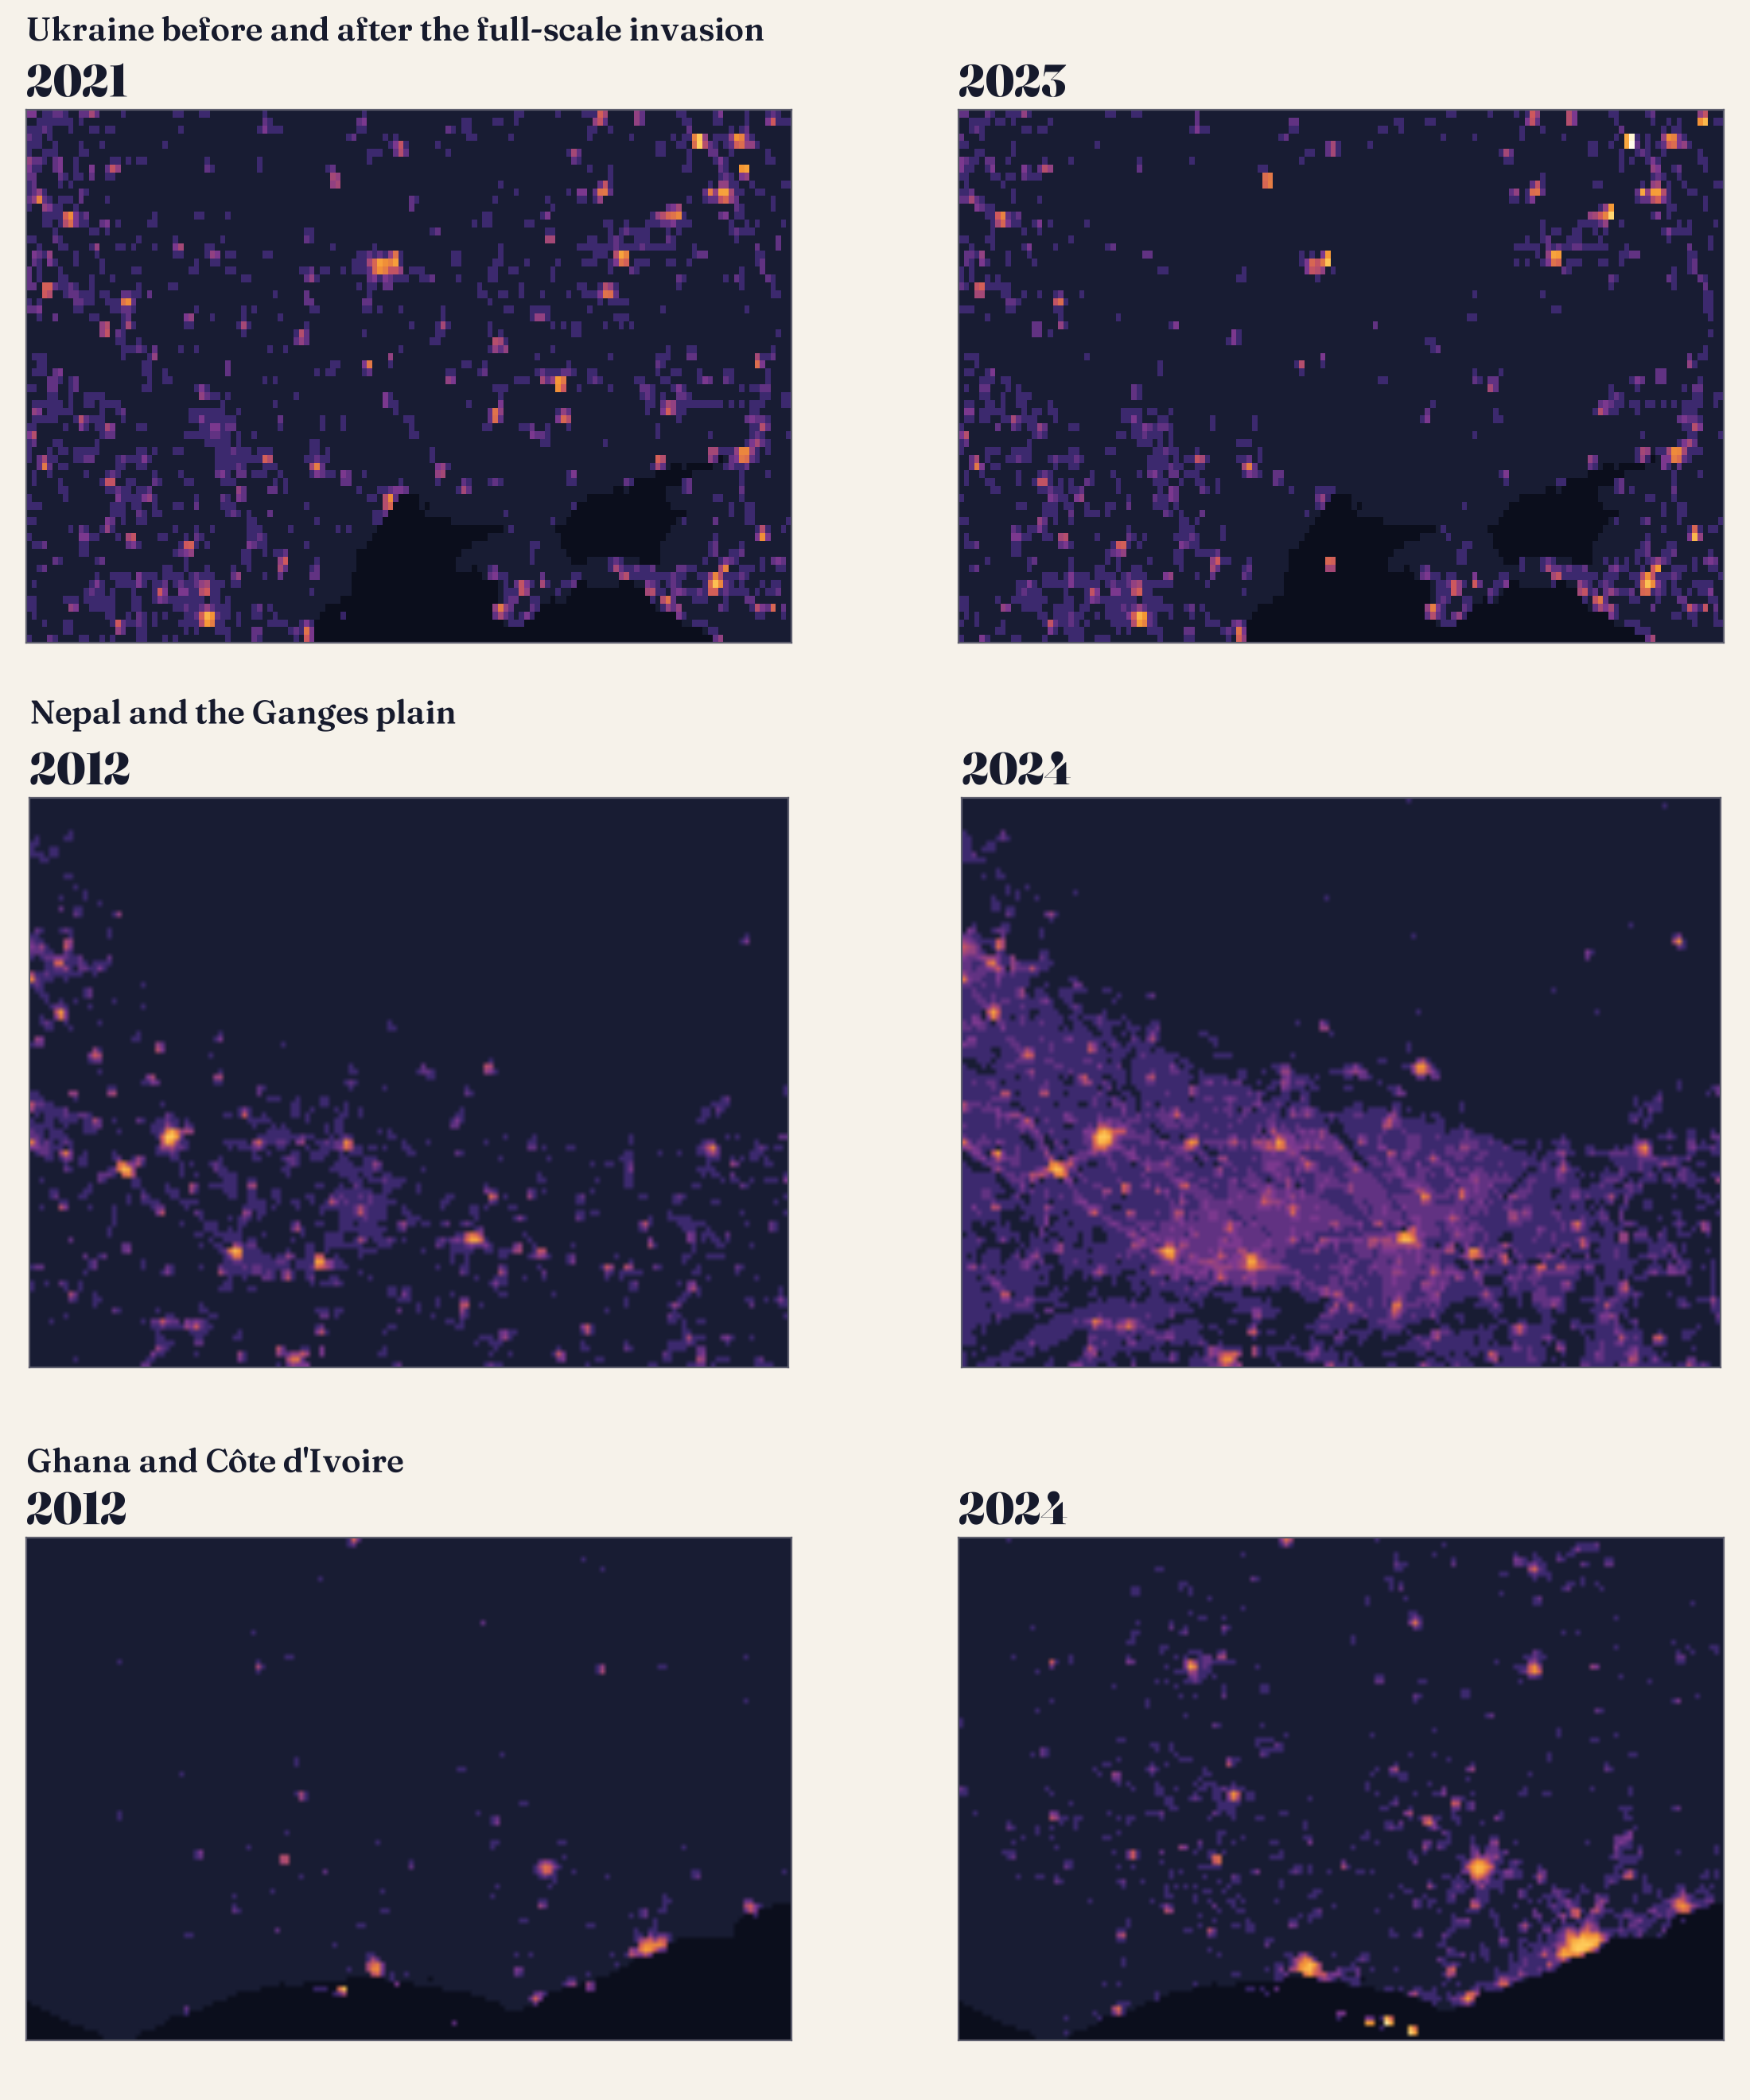
\includegraphics[width=.8\linewidth]{b_pairs.png}\caption{Before and after: Ukraine in 2021 and 2023 (15 km grid); Nepal and the Ganges plain, and Ghana and Côte d'Ivoire, in 2012 and 2024 (7 km grid).}\label{fig:pairs}\end{figure}

\subsection{Where it went dark}
17 of the 141 countries gave off less light in 2024 than in 2012, 12 of them by a tenth or more (Table~\ref{tab:down}). Three kinds of dimming can be told apart only from outside knowledge, not from the light itself.

\emph{War.} Ukraine's light fell 73\% between 2021 and 2022 and was 53\% below 2012 in 2024; Kharkiv lost 98\% of its light from its peak, Zaporizhzhia 96\% and Odesa 72\%. Syria lost a further 65\% between 2012 and 2015 and Aleppo 97\%, consistent with earlier analyses of the Syrian war from night lights \citep{li2014}. Yemen lost 68\% between 2012 and 2016 and Sanaa 95\%. Khartoum lost 77\% between 2022 and 2024, after fighting broke out in 2023. Mosul's light fell 70\% between 2013 and 2015 and recovered to 4.1 times its 2012 level by 2024 (Figure~\ref{fig:cities}).

\emph{Power and economic crises.} Lebanon lost 71\% of its light between 2019 and 2022, and Beirut 73\%. Venezuela lost 41\% between 2014 and 2020 (Maracaibo 53\%) before recovering, partly through flaring. Afghanistan lost 52\% between 2013 and 2022.

\emph{Changes in lighting.} France (-40\%), the Netherlands (-26\%), Switzerland (-19\%), the United Kingdom (-13\%) and Belgium (-10\%) dimmed without any comparable change in activity; Paris lost 24\% and London 24\%. The VIIRS Day/Night Band responds from about 500 to 900 nm and so misses much of the blue emission of white LEDs, which have been replacing high-pressure sodium street lamps \citep{kyba2017}; many towns now switch street lights off for part of the night, before the satellite's 1.30 am pass, and France's 2022 energy-saving rules required illuminated advertising to be off between 1 am and 6 am. Around The Hague (-60\%) and Rotterdam (-49\%) the fall is concentrated in the Westland greenhouse district, where artificial lighting was cut when gas prices rose in 2022. Ground-based observers report the night sky brightening by several per cent a year over a similar period \citep{kyba2023}, so these falls should not be read as darker nights.

\begin{table}[tbp]\centering\small\caption{Every ranked country whose light fell between 2012 and 2024.}\label{tab:down}\begin{tabular}{lrrrrl}\toprule Country & 2012 & 2024 & Change & 3-year & Deepest fall\\\midrule
Ukraine & 120.7 & 56.5 & -53\% & -58\% & 73\% (2021 to 2022)\\
Yemen & 71.7 & 33.7 & -53\% & -46\% & 68\% (2012 to 2016)\\
France & 658.1 & 393.5 & -40\% & -32\% & 46\% (2014 to 2024)\\
Syria & 95.6 & 58.0 & -39\% & -15\% & 65\% (2012 to 2015)\\
Netherlands & 229.9 & 169.5 & -26\% & -30\% & 33\% (2013 to 2022)\\
Estonia & 27.4 & 20.8 & -24\% & -5\% & 39\% (2021 to 2024)\\
Gabon & 23.9 & 18.5 & -23\% & -15\% & 35\% (2019 to 2023)\\
Afghanistan & 16.9 & 13.4 & -21\% & -34\% & 52\% (2013 to 2022)\\
Switzerland & 42.8 & 34.7 & -19\% & -15\% & 25\% (2013 to 2024)\\
Lebanon & 28.7 & 23.4 & -18\% & -42\% & 71\% (2019 to 2022)\\
United Kingdom & 438.8 & 381.1 & -13\% & -15\% & 20\% (2014 to 2024)\\
Belgium & 122.5 & 110.2 & -10\% & -14\% & 28\% (2020 to 2023)\\
Portugal & 190.4 & 182.7 & -4\% & -9\% & 18\% (2017 to 2022)\\
Puerto Rico & 44.9 & 44.3 & -1\% & -6\% & 25\% (2013 to 2017)\\
Uzbekistan & 126.0 & 125.4 & -1\% & +11\% & 36\% (2012 to 2016)\\
Egypt & 659.2 & 658.7 & -0\% & +4\% & 8\% (2021 to 2024)\\
Trinidad and Tobago & 34.2 & 34.2 & -0\% & -0\% & 9\% (2013 to 2016)\\
\bottomrule\end{tabular}\end{table}
\begin{figure}[tbp]\centering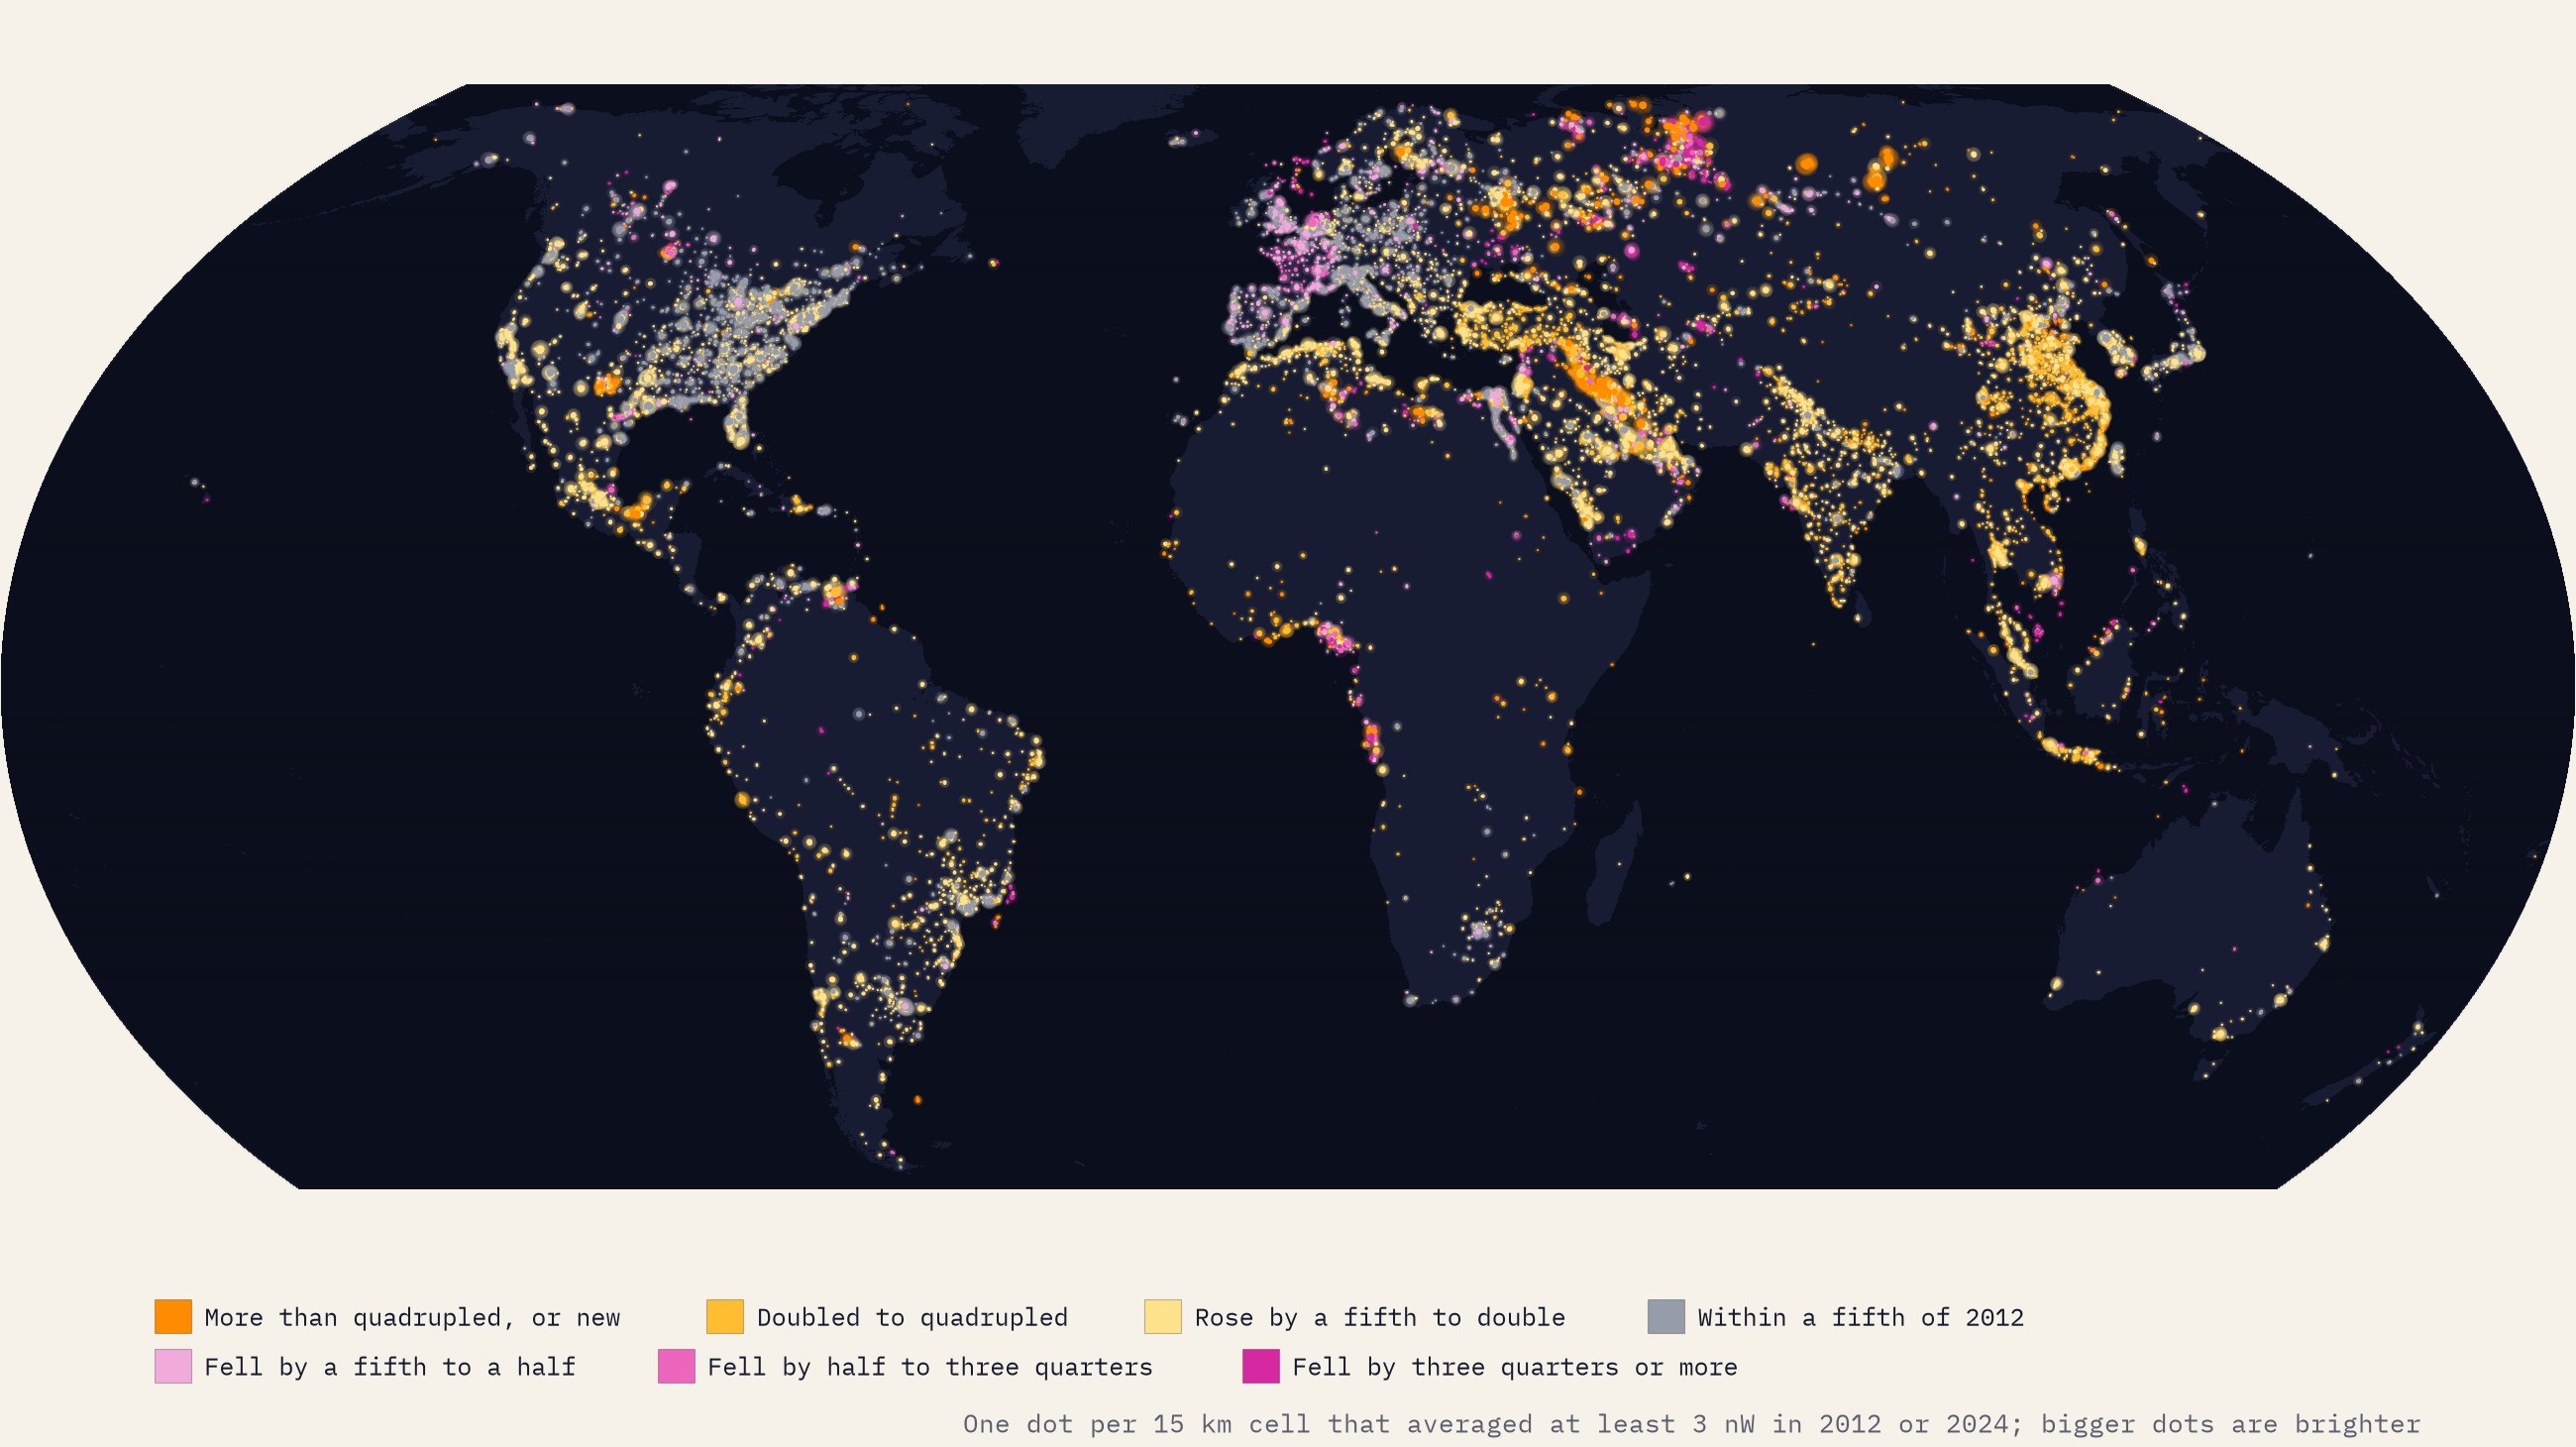
\includegraphics[width=\linewidth]{b_change_map.png}\caption{Change in light between 2012 and 2024: one dot per 15 km cell that averaged at least 3 nW in either year, coloured by the ratio of 2024 to 2012.}\label{fig:change}\end{figure}
\begin{figure}[tbp]\centering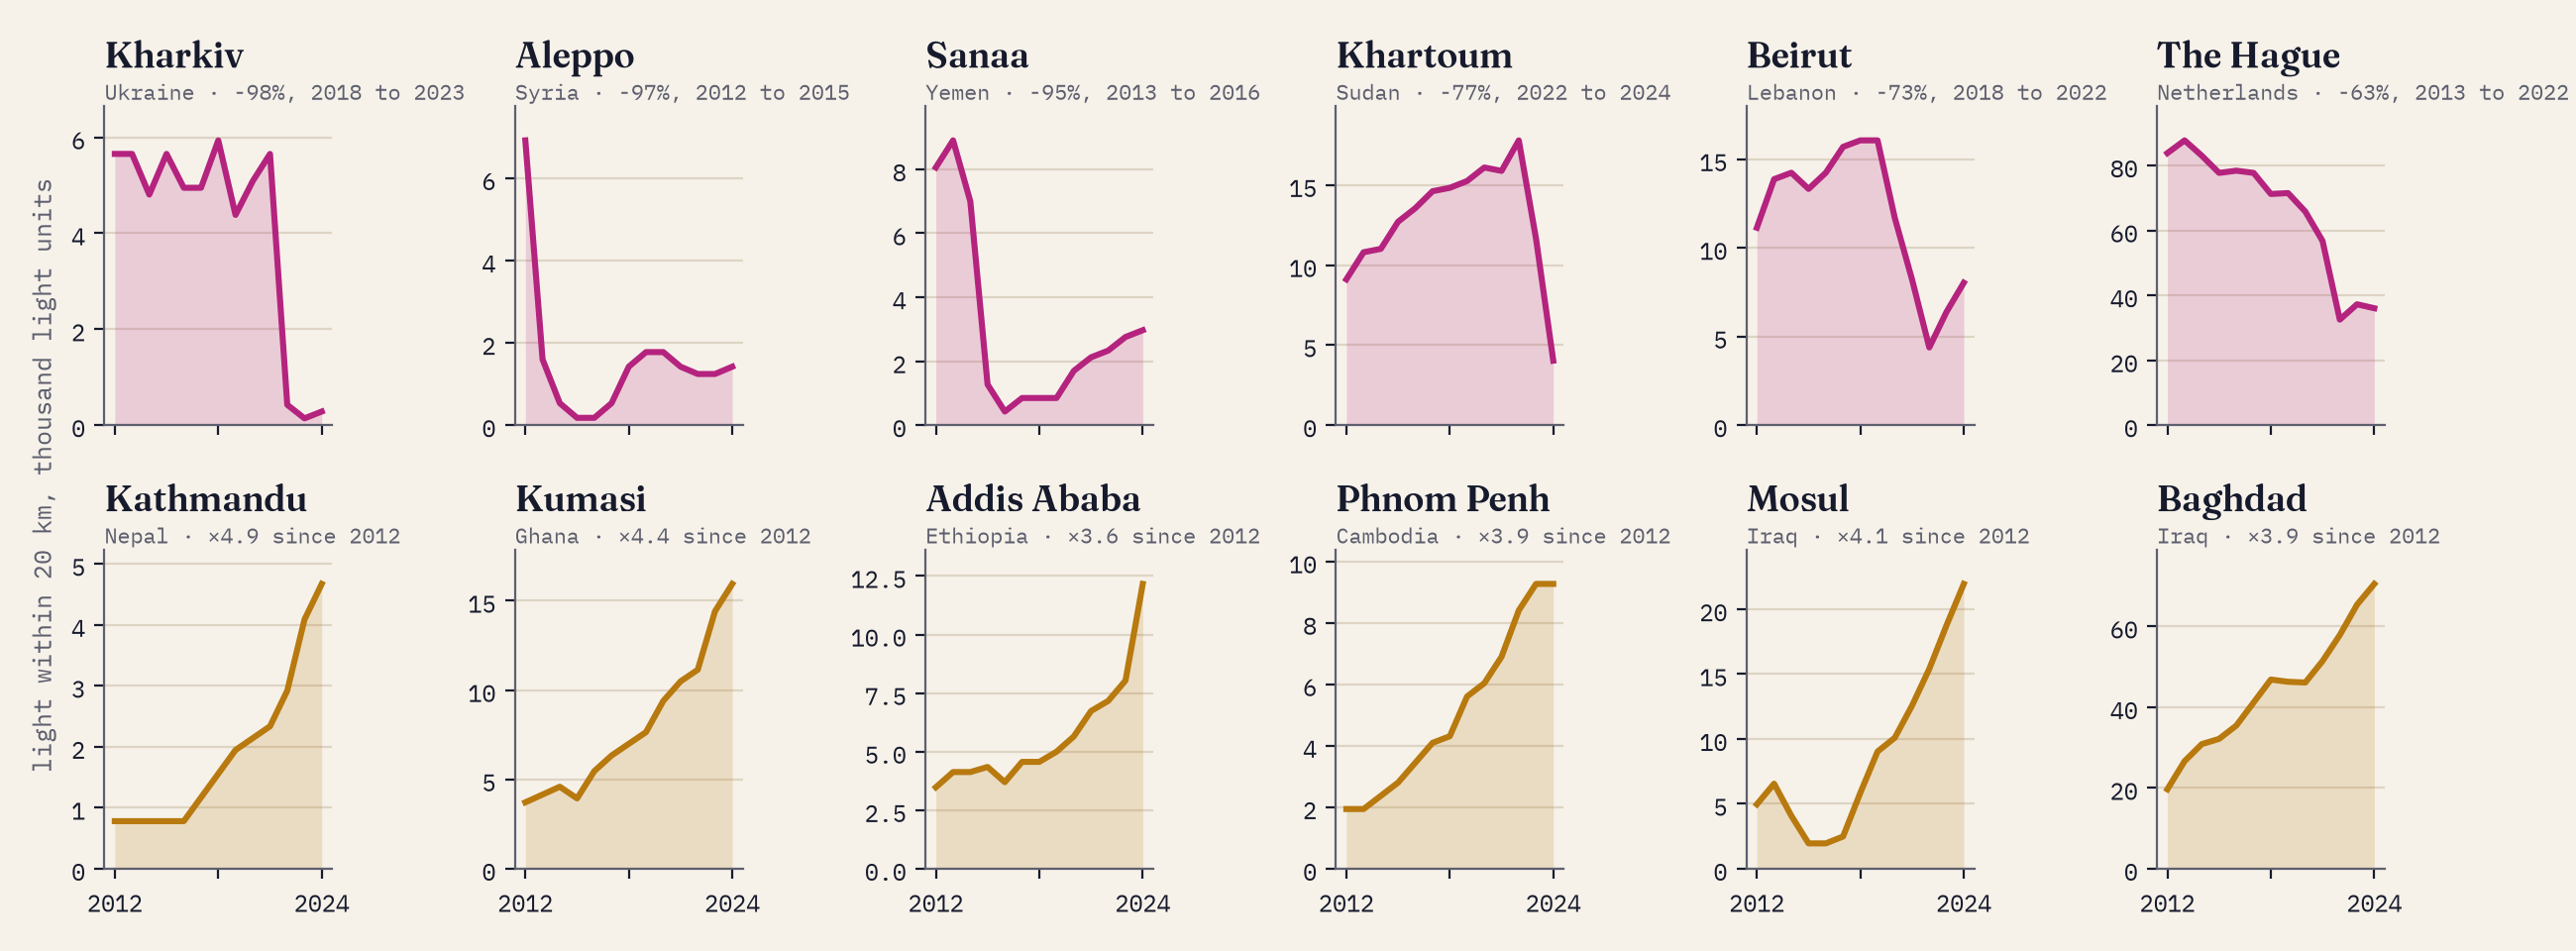
\includegraphics[width=\linewidth]{b_cities.png}\caption{Light within 20 km of twelve cities, 2012 to 2024 (15 km grid). Top: cities that went dark; bottom: cities that lit up.}\label{fig:cities}\end{figure}
\begin{table}[tbp]\centering\small\caption{Cities of a million or more whose light within 20 km changed most, 2012 to 2024 (7 km grid; discs that averaged at least 2 nW in 2012).}\label{tab:cities}\begin{tabular}{lrlr}\toprule Brightened & Change & Dimmed & Change\\\midrule
Kumasi, Ghana & +341\% & Kharkiv, Ukraine & -94\%\\
Mosul, Iraq & +310\% & Aleppo, Syria & -78\%\\
Baghdad, Iraq & +287\% & Sanaa, Yemen & -61\%\\
Addis Ababa, Ethiopia & +256\% & The Hague, Netherlands & -60\%\\
Lima, Peru & +248\% & Damascus, Syria & -59\%\\
Medan, Indonesia & +243\% & Rotterdam, Netherlands & -49\%\\
Haiphong, Vietnam & +237\% & Daqing, China & -43\%\\
Yerevan, Armenia & +230\% & Khartoum, Sudan & -41\%\\
Accra, Ghana & +228\% & Kyiv, Ukraine & -39\%\\
Nanchang, China & +204\% & Lille, France & -37\%\\
Dar es Salaam, Tanzania & +203\% & Omdurman, Sudan & -36\%\\
Abidjan, Ivory Coast & +202\% & Hyderabad, Pakistan & -32\%\\
\bottomrule\end{tabular}\end{table}

\subsection{Light per person}
With the world average at 100, Qatar scores 1,302, Libya 963 and Saudi Arabia 837; the United States 396, China 58 and India 37; Ethiopia 3.0, Uganda 5.0, DR Congo 5.5 and Bangladesh 5.8 (Figure~\ref{fig:pp}). By region, North America scores 392 and sub-Saharan Africa 18, a ratio of more than 21 to one. The top of the ranking mixes lit infrastructure with gas flaring and small populations.

\begin{figure}[tbp]\centering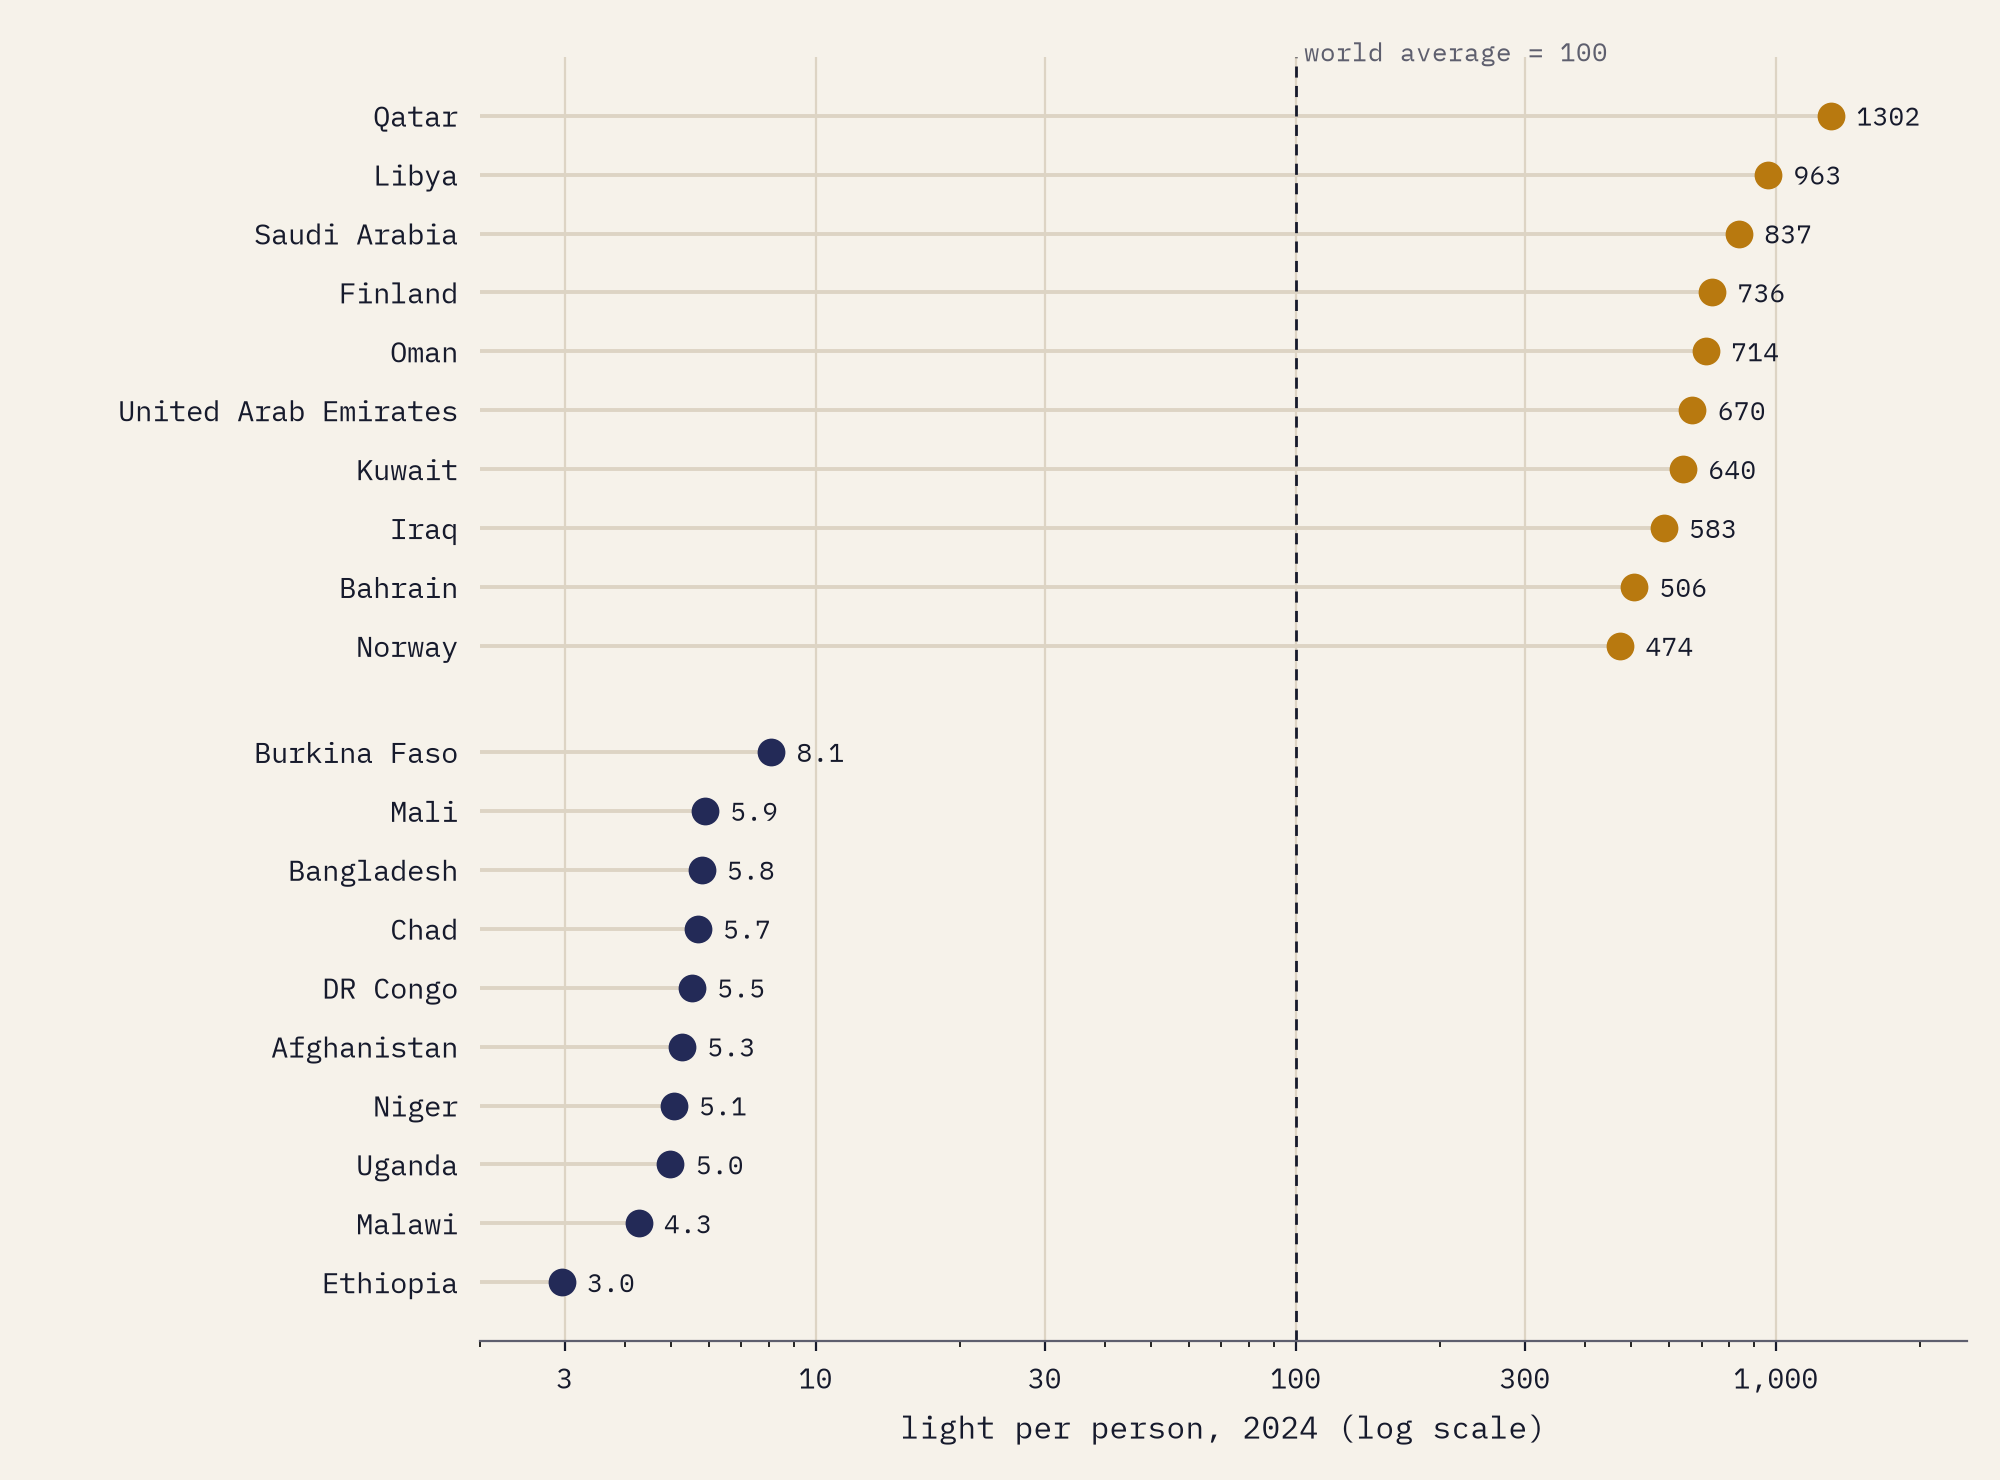
\includegraphics[width=.8\linewidth]{b_per_person.png}\caption{Light per person in 2024, world average = 100: the ten highest and lowest among countries with at least a million people.}\label{fig:pp}\end{figure}

\subsection{Robustness}
Comparing three-year averages instead of single years changes the direction of change for 6 of the 141 countries, each of them within a tenth of no change on one of the two measures; 19 countries fall on the three-year measure against 17 on single years.

\section{Limitations}
The annual composites are averages of cloud-free, moonless observations at about 1.30 am and say nothing about light earlier in the evening. The sensor's blindness to blue light biases trends downward wherever LEDs replace sodium lamps, and differently in different countries. Gas flares, greenhouses, mines and ports are counted with homes and streets. The 15 km and 7 km overview grids smooth small towns and blur city edges, and rounding to whole nW drops very faint light. Natural Earth populations are for about 2019 and its borders are de facto. City discs of fixed radius ignore city size and can overlap. The years 2000 to 2011 are a model, not observations; the DMSP-style layer is a long-term average; and a DMSP standard deviation layer in the extract used here was damaged and could not be read. Changes in light are associated with, not proof of, changes in electrification, economic activity or conflict.

\section*{Data availability}
Derived data (country, region, city and world tables, the page's map images and per-cell yearly values), all code and \texttt{results.json}, which holds every number quoted, are at \url{https://github.com/Tristan-Hotham/earth-at-night} and in the Zenodo record of this paper. The source rasters are available from \citet{hengl} under CC BY 4.0.

\section*{AI assistance}
I wrote the text, with drafting and editing assistance from Claude (Anthropic), which also helped prepare the analysis code. I reviewed and checked all text and results.

\begin{thebibliography}{99}
\bibitem[Elvidge et al.(2017)]{elvidge2017} Elvidge, C.D., Baugh, K., Zhizhin, M., Hsu, F.C. and Ghosh, T. (2017) VIIRS night-time lights. \emph{International Journal of Remote Sensing}, 38(21), 5860 to 5879.
\bibitem[Elvidge et al.(2021)]{elvidge2021} Elvidge, C.D., Zhizhin, M., Ghosh, T., Hsu, F.C. and Taneja, J. (2021) Annual time series of global VIIRS nighttime lights derived from monthly averages: 2012 to 2019. \emph{Remote Sensing}, 13(5), 922. doi:10.3390/rs13050922
\bibitem[Hengl(2025)]{hengl} Hengl, T. (2025) Annual time series of global VIIRS nighttime lights for 2000 to 2024 at 500 m spatial resolution extrapolated using logistic regression, version 0.4. Zenodo. doi:10.5281/zenodo.17294744 (concept record 10.5281/zenodo.7750174). CC BY 4.0.
\bibitem[Henderson et al.(2012)]{henderson} Henderson, J.V., Storeygard, A. and Weil, D.N. (2012) Measuring economic growth from outer space. \emph{American Economic Review}, 102(2), 994 to 1028.
\bibitem[Kyba et al.(2017)]{kyba2017} Kyba, C.C.M., Kuester, T., S\'anchez de Miguel, A., Baugh, K., Jechow, A., H\"olker, F., Bennie, J., Elvidge, C.D., Gaston, K.J. and Guanter, L. (2017) Artificially lit surface of Earth at night increasing in radiance and extent. \emph{Science Advances}, 3(11), e1701528.
\bibitem[Kyba et al.(2023)]{kyba2023} Kyba, C.C.M., Altinta\c{s}, Y.\"O., Walker, C.E. and Newhouse, M. (2023) Citizen scientists report global rapid reductions in the visibility of stars from 2011 to 2022. \emph{Science}, 379(6629), 265 to 268.
\bibitem[Li and Li(2014)]{li2014} Li, X. and Li, D. (2014) Can night-time light images play a role in evaluating the Syrian Crisis? \emph{International Journal of Remote Sensing}, 35(18), 6648 to 6661.
\bibitem[Li et al.(2020)]{li2020} Li, X., Zhou, Y., Zhao, M. and Zhao, X. (2020) A harmonized global nighttime light dataset 1992 to 2018. \emph{Scientific Data}, 7, 168. doi:10.1038/s41597-020-0510-y
\bibitem[Natural Earth(2026)]{ne} Natural Earth (2026) Admin 0 countries and populated places, 1:10m. naturalearthdata.com. Public domain.
\end{thebibliography}
\end{document}
